\documentclass[useAMS, usenatbib, a4paper]{mnras}
\pdfsuppresswarningpagegroup=1
\usepackage[spanish,es-minimal,english]{babel}
\usepackage[utf8]{inputenc}
\usepackage{graphicx}
\let\Bbbk\relax
\usepackage{amsmath}	% Advanced maths commands
\usepackage{amssymb}	% Extra maths symbols
\usepackage{xcolor}
\usepackage{fixltx2e}
\usepackage{hyperref}
\usepackage{savesym}
\savesymbol{tablenum}
\usepackage{siunitx}
\restoresymbol{SIX}{tablenum}
\usepackage{newtxtext}
\usepackage[varg,varvw,smallerops]{newtxmath}
\usepackage{xfrac} % for the \sfrac macro
\usepackage{booktabs}
\usepackage{longtable}
\usepackage{array}   % for \newcolumntype macro
\newcolumntype{L}{>{$}l<{$}} % math-mode version of lrc column types
\newcolumntype{R}{>{$}r<{$}} 
\newcolumntype{C}{>{$}c<{$}}
\hypersetup{colorlinks=True, linkcolor=blue!50!black, citecolor=black,
  urlcolor=blue!50!black}
\usepackage{etoolbox}
\robustify\bfseries
\robustify\itshape
\usepackage{enumerate}
\bibliographystyle{mnras}
\sisetup{
  % explicit""+" is useful for velocities
  retain-explicit-plus = true,
  % prefer 10^6 over 1 x 10^6
  retain-unity-mantissa = false,
  % Use x +/- e instead of x(e)  
  separate-uncertainty = true,
  % Make sure to pick up bold font when used in section heading for instance
  detect-weight = true,
  table-align-uncertainty = true,
  table-align-comparator = true,
}
\DeclareSIUnit\msun{\text{M\ensuremath{_\odot}}}
\DeclareSIUnit\lsun{\text{L\ensuremath{_\odot}}}
\DeclareSIUnit\zsun{\text{Z\ensuremath{_\odot}}}
\DeclareSIUnit\angstrom{\text{\AA}}

% A better \ion command that works in more circumstances
\newcommand\ION[2]{#1\,\scalebox{0.9}[0.8]{\uppercase{#2}}}
\newcounter{ionstage}
\renewcommand{\ion}[2]{\setcounter{ionstage}{#2}% 
  \ensuremath{\mathrm{#1\,\scriptstyle\Roman{ionstage}}}}
\newcommand\hii{\ion{H}{2}}



\newcommand\wind{\ensuremath{_{\mathrm{w}}}}
\newcommand\mdwind{\ensuremath{\dot M\wind}}
\newcommand\orb{\ensuremath{_{\mathrm{o}}}}
\newcommand\rel{\ensuremath{_{\mathrm{r}}}}
\newcommand\Hill{\ensuremath{_{\mathrm{\scriptscriptstyle H}}}}
\newcommand\bhl{\ensuremath{_{\mathrm{\scriptscriptstyle B}}}}
\newcommand\Tej{\ensuremath{_{\mathrm{\scriptscriptstyle T}}}}
\newcommand\acc{\ensuremath{_{\mathrm{acc}}}}
\newcommand\mdacc{\ensuremath{\dot M\acc}}
\newcommand\qq{\ensuremath{\tilde{q}}}
\title[Wind accretion in a circular binary system]
{
  Wind accretion in a circular binary system  
}

\author[Henney et al.]{
  William J. Henney\textsuperscript{1}\thanks{w.henney@irya.unam.mx}
  \\
  \textsuperscript{1}\foreignlanguage{spanish}{%
    Instituto de Radioastronomía y
    Astrofísica, Universidad Nacional Autónoma de México, Apartado
    Postal 3-72, 58090 Morelia, Michoacán, Mexico}\\
}


% These dates will be filled out by the publisher
\date{Accepted XXX. Received YYY; in original form ZZZ}

% Enter the current year, for the copyright statements etc.
\pubyear{2024}


\begin{document}
\label{firstpage}
\pagerange{\pageref{firstpage}--\pageref{lastpage}}
\maketitle



\begin{abstract}
  Commentary on \citet{Tejeda:2025a}.
\end{abstract}

\begin{keywords}
Binary stars -- stellar winds -- stellar accretion
\end{keywords}
%\facilities{VLT:Yepun (MUSE); OANSPM:2.1m (Mezcal); Keck (HIRES)}
%\object{M42}

\section{Introduction}
\label{sec:introduction}

\section{Binary system and wind parameters}
\label{sec:binary-syst-param}

Consider a binary system in which the secondary star with mass \(M_2\) accretes from the wind of the primary star with mass \(M_1\).
The orbit is assumed to be circular with separation \(r\).
The orbital speed of the secondary in the rest frame of the primary is \(v\orb\).
Kepler's laws gives the orbital period \(T\) as
\begin{equation}
  \label{eq:period}
  T = 2\pi G \bigl(M_1 + M_2\bigr) / v\orb^3 = 2\pi r / v_0. 
\end{equation}

The isotropic stellar wind from the primary has mass-loss rate \(\dot M\wind\) and hypersonic terminal velocity \(v\wind\).
The undisturbed wind density \(\rho\wind\) at the position of the secondary is therefore
\begin{equation}
  \label{eq:rho-wind}
  \rho\wind = \mdwind / 4\pi r^2 v\wind. 
\end{equation}

The orbital velocity is purely tangential and thus perpendicular to the purely radial wind velocity. The relative speed between the wind and the secondary star is therefore
\begin{equation}
  \label{eq:relative-velocity}
  v\rel = \Bigl(v\wind^2 + v\orb^2\Bigr)^{1/2}.
\end{equation}

The system is characterized by two dimensionless parameters:
\begin{equation}
  \label{eq:mass-ratio}
  \text{Mass ratio:}\quad q \equiv M_2 / \bigl(M_1 + M_2\bigr),
\end{equation}
\begin{equation}
  \label{eq:velocity-ratio}
  \text{Velocity ratio:}\quad w \equiv v\wind / v\orb.
\end{equation}

\section{Bondi--Hoyle--Lyttleton (BHL) accretion}
\label{sec:bondi-hoyle-lyttl}

\begin{figure}
  \centering
  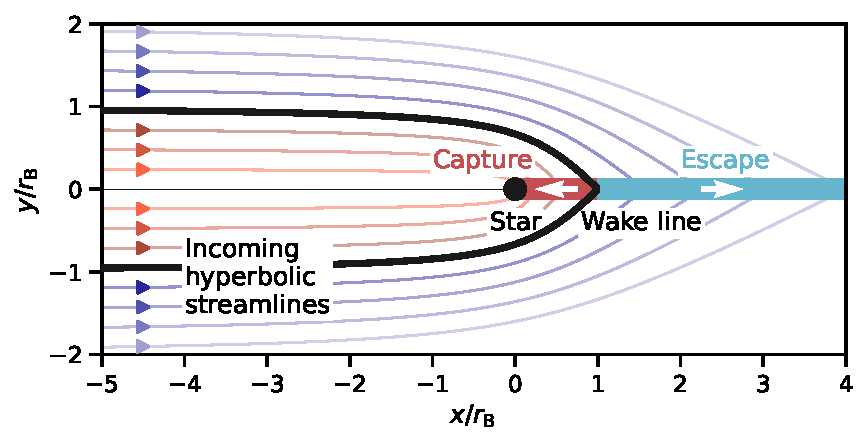
\includegraphics[width=\linewidth]{notebooks/hoyle-lyttleton-trajectories}
  \caption{Bondi--Hoyle--Lyttleton model for accretion}
  \label{fig:bhl}
\end{figure}
Following \citet{Hoyle:1939a, Bondi:1944a},
the mass accretion rate is
\begin{equation}
  \label{eq:mdot-bhl}
  \mdacc = \pi r\bhl^2 \, v\rel \, \rho\wind , 
\end{equation}
where
\begin{equation}
  \label{eq:radius-bhl}
  r\bhl = 2 G M_2 / v\rel^2 
\end{equation}
is the accretion radius.
From equations~(\ref{eq:period}, \ref{eq:relative-velocity}, \ref{eq:mass-ratio}, \ref{eq:velocity-ratio}) we find that the ratio of the accretion radius to the orbital radius is
\begin{equation}
  \label{eq:racc-over-r}
  r\bhl / r = 2 q / \bigl(1 + w^2\bigr).
\end{equation}

We define a dimensionless accretion efficiency as the fraction of the stellar wind that is captured by the secondary:
\begin{equation}
  \label{eq:eta-bhl-def}
  \eta\bhl \equiv \mdacc / \mdwind ,
\end{equation}
which from equations~(\ref{eq:rho-wind}, \ref{eq:mdot-bhl}) yields
\begin{equation}
  \label{eq:eta-bhl}
  \eta\bhl = \frac{1}{4}
  \biggl( \frac{v\rel}{v\wind} \biggr)
  \biggl( \frac{r\bhl}{r}\biggr)^2 . 
\end{equation}
The boost of the relative wind speed due to the orbital motion is
\begin{equation}
  \label{eq:boost-ratio}
  v\rel / v\wind =  w^{-1} \, \bigl(1 + w^2\bigr)^{1/2} ,
\end{equation}
which combine with equations~(\ref{eq:eta-bhl}, \ref{eq:racc-over-r}) implies
\begin{equation}
  \label{eq:eta-bhl-dimensionless}
  \eta\bhl = \frac{q^2}{w \, \bigl(1 + w^2\bigr)^{3/2}} .
\end{equation}

The BHL analysis assumes that the wind density and velocity vector are constant
over the entire accretion capture zone of radius \(r\bhl\).
For accretion from a wind, this is only true in the limit that
\(r\bhl \ll r\). 

\section{A problematic geometric correction}
\label{sec:Tejeda-geometry}

\cite{Tejeda:2025a} point out an issue with equation~(\ref{eq:eta-bhl-dimensionless}) when the wind velocity is much smaller than the orbital velocity (\(w \ll 1\)): in the limit \(w \to 0\) then \(\eta\bhl \to q^2 / w\), which can become larger than unity.
This is clearly non-physical since the mass accretion rate cannot exceed the wind mass-loss rate.
They propose to remedy this deficiency by making a geometric correction
to the mass accretion rate.
\(\mdacc\) is multiplied by a factor of \(\cos\theta\),
where \(\theta\) is the angle between the relative velocity vector
and the radial direction from the primary,
which accounts for
\begin{center}
  \begin{minipage}{0.8\linewidth}\small\itshape
    \dots the projected area of the accretion cylinder's
    cross section onto a sphere centered around the primary. This
    projection accounts for the effective area capturing the wind.
  \end{minipage}
\end{center}
This yields a different equation for the accretion efficiency:
\begin{equation}
  \label{eq:eta-tejeda-dimensionless}
  \eta\Tej = \eta\bhl = \biggl( \frac{q}{1 + w^2} \biggr)^2 .
\end{equation}
This clearly resolves the issue mentioned above since as
\(w \to 0\) then \(\eta\Tej \to q^2 \), guaranteeing that \(\eta\Tej < 1  \).
On the other hand, in the opposite limit of large wind velocity
the two efficiencies agree: as \(w \to \infty\) then \(\eta\Tej \to \eta\bhl \to q^2 / w^4\).

However, the physical basis for making this ``correction'' is unclear.
Unlike the BHL theory, which is entirely local
to the rest frame of the accreting secondary,
the correction factor introduces quantities from the rest frame of the primary,
which casts doubt on its validity.

For circular orbits, one finds
\begin{equation}
  \label{eq:cos-theta}
  \cos\theta = v\wind / v\rel ,
\end{equation}
so an alternative way of writing the Tejeda efficiency is
\begin{equation}
  \label{eq:eta-tejeda}
  \eta\Tej = \frac{1}{4}
  \biggl( \frac{r\bhl}{r}\biggr)^2
  =  \frac{\pi \, r\bhl^2}{4 \pi \, r^2} ,
\end{equation}
which is simply the area covering factor of the BHL capture zone
of a \emph{stationary} accretor.
However, this is inconsistent with the well-defined physical limit
for a fast-orbiting accretor, as we will show in the following section.

\section{Asymptotic efficiency of a fast-orbiting accretor in a slow wind}
\label{sec:fast-orbit-accr}

During one orbital period, \(T\),
the accretion capture zone will sweep out a torus that
fully encircles the primary star.
If \(T\) is sufficiently short compared with the time \(2 r\bhl \sin \theta / v\wind\) for the wind to cross the accretion capture zone, then all of the wind that passes within
a distance \(r\bhl\) of the orbital path will be captured.
This corresponds to the limit \(w \ll 1\), \(\theta \approx \pi/2\), for which
the solid angle subtended at the primary by the torus is
\begin{equation}
  \label{eq:omega-torus}
  \Omega = 2 \pi \int_{-r\bhl / r}^{r\bhl / r} d\mu = 4 \pi \, r\bhl / r
\end{equation}
Therefore, the limiting accretion efficiency is
\begin{equation}
  \label{eq:1}
  \eta_{\lim} = \Omega / 4\pi = \lim_{w \to 0} \frac{r\bhl}{r} = 2 q .
\end{equation}
Note that this is inconsistent with the Tejeda result,
\(\eta\Tej \approx q^2\), in the same limit, casting further doubt on
the correctness of that result.

It is also inconsistent with the naive BHL result, \(\eta\bhl \to \infty\),
so we clearly require \emph{some} correction to BHL.
In the following section we outline a physically motivated correction
that is consistent with \(\eta_{\lim}\).

\section{Starvation by finite refill time}
\label{sec:starv-finite-refill}

\begin{figure}
  \centering
  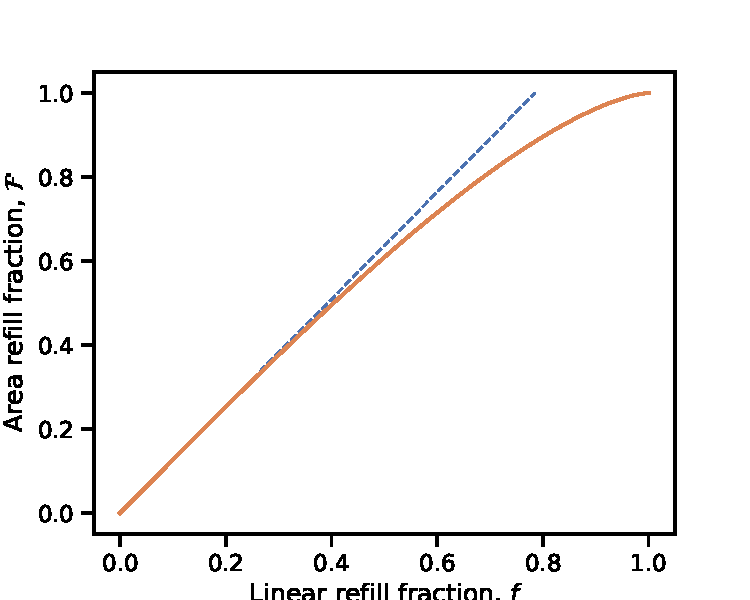
\includegraphics[width=\linewidth]{notebooks/refill-fraction}
  \caption{Refill fraction of the accretion surface area \(\mathcal{F}\)
    from equation~(\ref{eq:refill-area-fraction}).
    The dashed line shows the linear approximation \(\mathcal{F} = 4 f / \pi\).
  }
  \label{fig:area-F}
\end{figure}

\begin{figure}
  \centering
  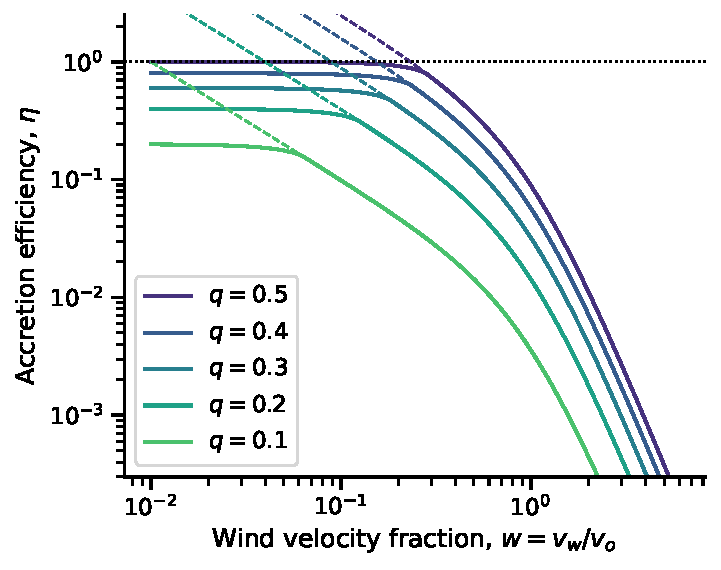
\includegraphics[width=\linewidth]{notebooks/eta-finite-refill}
  \caption{
    Accretion efficiency \(\eta_\star\) accounting for finite refill time (solid lines)
    from equations~(\ref{eq:refill-linear-fraction}, \ref{eq:refill-area-fraction}, \ref{eq:eta-refill}).
    Dashed lines show the naive BHL efficiency \(\eta\bhl\) from
    equation~(\ref{eq:eta-bhl-dimensionless}).
  }
  \label{fig:eta-finite-refill}
\end{figure}


\cite{Tejeda:2025a} discuss the refill time, which is the time
needed for the wind to replenish the material inside the accretion torus
(see previous section)
but they do not explicitly calculate its influence on the accretion efficiency.
However, we will show that accounting for this effect is entirely sufficient
to prevent the divergence of \(\eta\bhl\) for small \(w\).

During a single orbital period, the wind will propagate a distance
\begin{equation}
  \label{eq:wind-propagation}
  x = v\wind T = 2\pi w r ,
\end{equation}
where the second equality makes use of
equations~(\ref{eq:period}, \ref{eq:velocity-ratio}).
The radial thickness in the orbital plane of the accretion torus
can be found by applying the cosine law and
Taylor expansion in powers of \(r\bhl / r\) to yield
\begin{equation}
  \label{eq:torus-thickness-taylor}
  h = 2 r\bhl \sin\theta
  \biggl[
  1 - \frac12 \bigl( r\bhl / r \bigr)^2 \cos^2\theta 
  + \mathcal{O} \bigl( r\bhl / r \bigr)^4
  \biggr].
\end{equation}
For small \((r\bhl / r) \cos\theta\) the term in square brackets is approximately unity,
so from equations~(\ref{eq:boost-ratio}, \ref{eq:cos-theta}) we have
\begin{equation}
  \label{eq:torus-thickness-approx}
  h \approx 2 r\bhl \sin\theta = 2 r\bhl \bigl(1 + w^2\bigr)^{-1/2}.
\end{equation}
Therefore the fraction of the thickness refilled by the wind is
\begin{equation}
  \label{eq:refill-linear-fraction}
  f = x / h = \frac{\pi w \bigl(1 + w^2\bigr)^{3/2}}{2 q}. 
\end{equation}
If \(f < 1\), then a portion of the accretion surface \(\pi r\bhl^2\) is empty of wind,
resulting in a reduction in the effective area by a factor \(\mathcal{F}\),
which can be found for small \((r\bhl / r)\) from the standard formula
for the area of a circular segment, yielding
\begin{equation}
  \label{eq:refill-area-fraction}
  \mathcal{F} = 1 - \frac{2}{\pi} \biggl[
  \cos^{-1} (f) \, - \, f\, \bigl(1 - f^2 \bigr)^{1/2}
  \biggr]
  \approx \frac{4 f}{\pi} 
  ,
\end{equation}
where the final approximate equality is accurate for \(f \la 0.4\).
This function is shown in Figure~\ref{fig:area-F}.

In this refill-limited case, the accretion efficiency is therefore given
from equations~(\ref{eq:eta-bhl-dimensionless}, \ref{eq:refill-linear-fraction},
\ref{eq:refill-area-fraction}) as
\begin{equation}
  \label{eq:eta-refill}
  \eta_{\star} = \mathcal{F} \eta\bhl \approx 2 q ,
\end{equation}
which applies when \(w \la 0.64 q\).
Note that this is exactly the same efficiency as the limiting value
\(\eta_{\lim}\) from section~\ref{sec:fast-orbit-accr}.
We have therefore shown how the asymptotic behavior of the accretion efficiency
when the wind speed is small compared with the orbital speed
can arise naturally from a reduction in the accretion area due to
the ``hole'' in the wind that was cleared out during the previous orbit.
By using the exact expression for \(\mathcal{F} \) in equation~(\ref{eq:refill-area-fraction}),
we achieve a smooth transition from \(\eta_{\star}\) to \(\eta\bhl\) for \(w > q\).
The resultant efficiency is plotted against \(w\) for different
values of \(q\) in Figure~\ref{fig:eta-finite-refill}. 

\begin{figure}
  \centering
  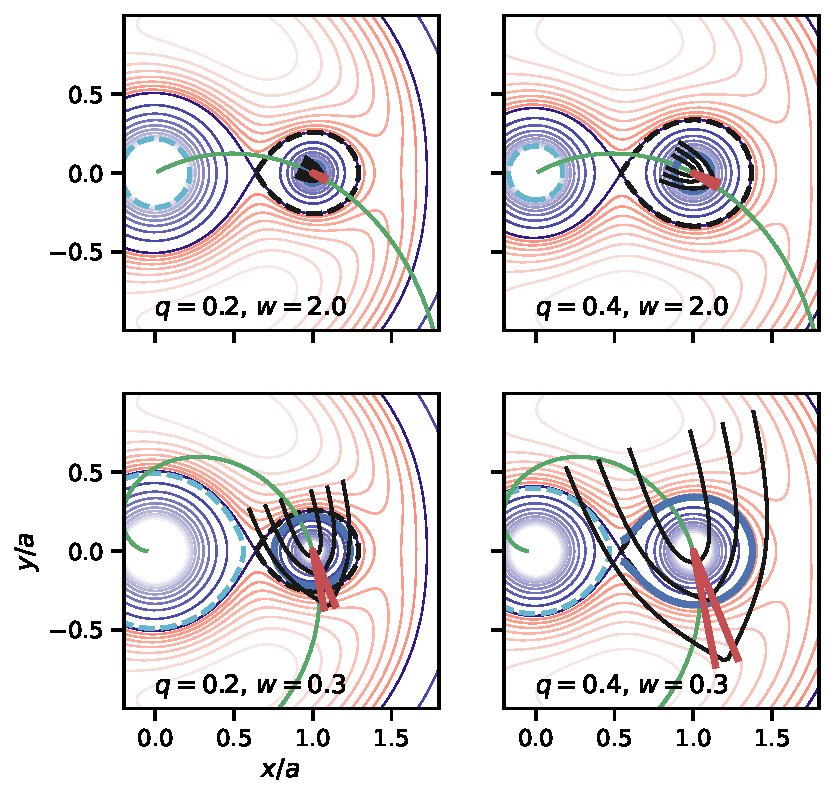
\includegraphics[width=\linewidth]{notebooks/roche-potential-trajectories}
  \caption{
    Effective potentials and wind trajectories in rotating frame.
  }
  \label{fig:roche-potential-trajectories}
\end{figure}

\section{Gravitational influence of the primary}
\label{sec:limit-hill-sphere}
\begin{figure}
  \centering
  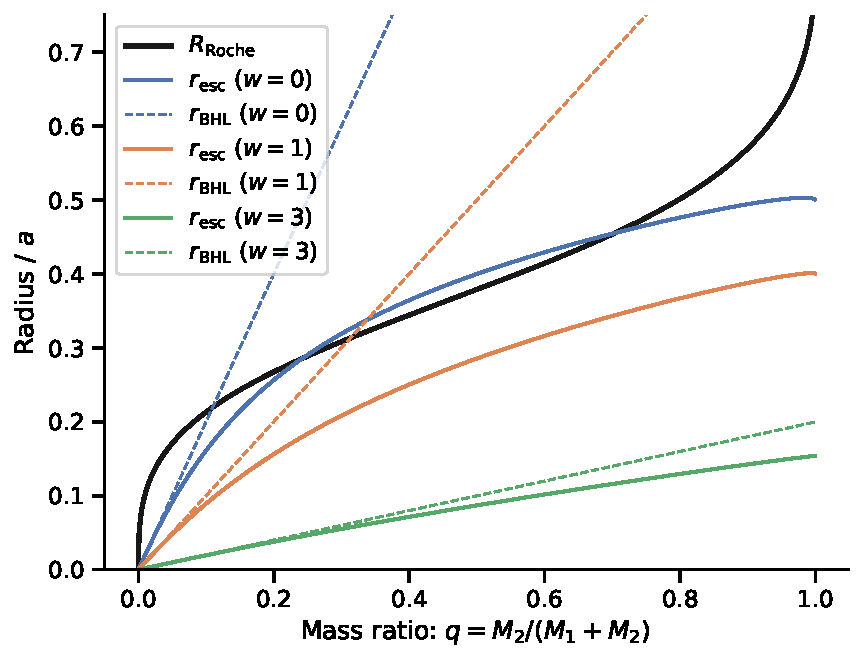
\includegraphics[width=\linewidth]{notebooks/roche-escape-L4-radii-vs-q}
  \caption{
    Gravitational escape radii (solid lines) as function of mass ratio,
    \(q\), and for different values of the wind-to-orbital speed ratio, \(w\).
    These correspond to the minimum radius around the secondary where the inflowing wind
    has enough kinetic energy to escape past the \(L_4, L_5\) potential maximum.
    The corresponding BHL values for an isolated accretor are shown dashed lines.
    The thick solid black line shows the equivalent-volume radius of the Roche surface. 
  }
  \label{fig:escape-radii}
\end{figure}

\begin{figure}
  \centering
  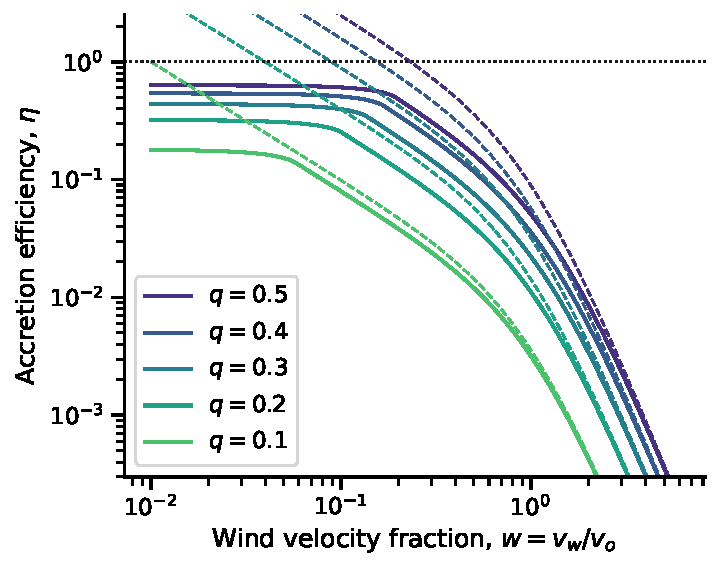
\includegraphics[width=\linewidth]{notebooks/eta-roche-finite-refill}
  \caption{
    Same as Figure~\ref{fig:eta-finite-refill} but
    also accounting for tidal perturbation by the primary. 
    Dashed lines show the naive BHL efficiency \(\eta\bhl\) from
    equation~(\ref{eq:eta-bhl-dimensionless}).
  }
  \label{fig:eta-tidal-perturbation}
\end{figure}




The derivation of the Bondi--Hoyle-Lyttleton accretion rate
(section~\ref{sec:bondi-hoyle-lyttl})
treats the gravity of the accreting star in isolation.
However, in a binary system this is only valid within the
``gravitational sphere of influence'' of the secondary
\citetext{\citealp{Souami:2020a} and references therein}.
We will quantify this by considering equipotential
surfaces in the rotating frame of the binary orbit,
which are characterized by the five equilibrium Lagrange points
\(L_1\) to \(L_5\).
The gravitational attraction of the secondary dominates
over tidal perturbations only within the Roche surface
of the secondary, which 
which extends between the Lagrange points \(L_1\) and \(L_2\),
see Figure~\ref{fig:roche-potential-trajectories}.

Following \citet{Seidov:2004a},
the effective potential in the rotating frame
can be written in non-dimensional form as
\begin{multline}
  \label{eq:effective-potential}
  U(x, y, z) = (x - q)^2 + y^2               % centrifugal
  + \frac{-2 (1 - q) (1 - \Gamma)}{\bigl(x^2 + y^2 + z^2\bigr)^{1/2}} \\ % primary
  + \frac{-2 q}{\bigl((x-1)^2 + y^2 + z^2\bigr)^{1/2}}   % secondary
\end{multline}
where \((x, y, z)\) are orthogonal Cartesian coordinates
in units of the binary separation, \(a\),
with origin at the position of the primary star. The orbit lies in the \(xy\) plane,
with the secondary located at \((x, y, z) = (1, 0, 0)\).\footnote{%
  Note that the mass ratio \(q = M_2 / (M_1 + M_2)\) used in this paper differs from that
  employed in some of the binary star literature, which we denote \(\qq = M_2 / M_1\)
  with the conversion \(\qq = q / (1 - q)\).
}
The potential \(U\) is in units of \(G (M_1 + M_2) / (2 a) = \frac12 \Omega^2\), where \(\Omega = 2 \pi / P = v\orb / a\) is the orbital angular velocity.
The acceleration of the primary's wind due to radiation pressure on dust grains is
accounted for by an effective Eddington factor \(\Gamma = L_1 / L_{\mathrm{Edd}}\), but we will initially set \(\Gamma = 0\). 


\bibliography{accretion-refs}

\appendix

\section{Details of Hoyle--Lyttleton accretion}
\label{sec:deta-hoyle-lyttl}



% Don't change these lines
\bsp	% typesetting comment
\label{lastpage}

\end{document}

%%% Local Variables:
%%% mode: LaTeX
%%% TeX-master: t
%%% End:
